%% *** TODO ***
%% cerca bib: e completa
\documentclass[a4paper, 11pt]{article}
\usepackage[T1]{fontenc}
\usepackage[utf8]{inputenc}
\usepackage{graphicx}
\usepackage{hyperref}

\hypersetup{
    pdfborder={0 0 0}
}

\newcommand{\code}[1]{\texttt{#1}}
\newcommand{\issue}[3][?]{
    \paragraph{[#1] #2} \mbox{}\\ #3
}
\begin{document}

\title{Code inspection}


\author{M. Albanese, M. Bianchi, A. Carlucci}

\maketitle
\newpage{}
\tableofcontents{}

\newpage{}


\section{Description of classes}

The \code{RealmAdapter} class provides authentication and authorization functionalities
to access web resources. In particular, its role is to let users login,
logout and to check users privileges.

The class is contained in the package \code{com.sun.web.security} which mainly
contains:
\paragraph{HTTP wrappers} \mbox{} \\  
\code{HttpRequestWrapper.java} and \code{HttpResponseWrapper.java}.


\paragraph{Helper login functions} \mbox{} \\ 
\code{LoginProbeProvider.java} and \code{LoginStatsProvider.java}

\paragraph{SSL Factory} \mbox{} \\ 
\code{SSLSocketFactory.java} 

\newpage
\section{Functional roles of the assigned class}
Java EE provides an elaborate security system to provide access to protected resources on the web server. According to official documentation (see~\cite{bib:docurl}):

\begin{quotation}
    Java EE applications consist of components that can contain both protected and unprotected resources. Often, you need to protect resources to ensure that only authorized users have access. \emph{Authorization provides controlled access to protected resources}. \\
    Authorization is based on identification and authentication. \\
    \textbf{Identification} is a process that enables recognition of an entity by a system. \\
    \textbf{Authentication} is a process that verifies the identity of a user, device, or other entity in a computer system, usually as a prerequisite to allowing access to resources in a system.
\end{quotation}

The main function for this class is to provide code that guarantees what stated above; in other words, code for \emph{authentication} and \emph{logout}, \emph{authorization}, \emph{role checking}.

\subsection{Authentication}
The whole set of protected resources is partitioned into security spaces called \textbf{realms}, characterized by security policies and allowed users/groups. There are two important predefined realms in Java EE:
\begin{itemize}
    \item \code{file}: check inserted credentials with the ones contained in a \code{keyfile};
    \item \code{certificate}: an \code{X.509} certificate is provided by the client through an \code{HTTPS} connection, which is verified on the server side.
\end{itemize}

The class \code{RealmAdapter} wraps auth functionalities both via credentials and certificates by using several overloaded \code{authenticate()} functions and logout functionalities through a \code{logout()} method. In particular, each \code{authenticate()} delegates to the one in line 676 (described in section~\ref{sub:auth}).

\subsection{Users, groups, roles and principals}
\begin{figure}[tb]
    \centering
    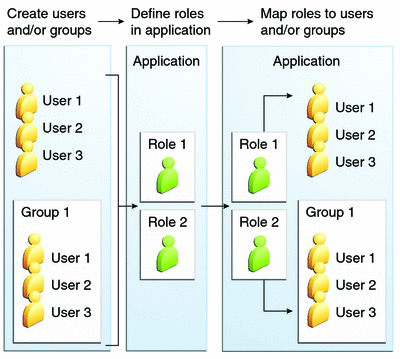
\includegraphics[]{img/security.png}
    \caption{Mapping between users and roles}
    \label{fig:security}
\end{figure}

The actual recognition of customers on the server is OS-like: the ones defined in the system are called \textbf{users} and can either be humans or applications. Multiple users can belong to the same \textbf{group}, which is a useful subdivision when several people are involved (e.g. an e-commerce site could contain a \code{CUSTOMER} group defined). In a similar fashion, \textbf{roles} define a division of users; they differ in the \emph{scope}:
\begin{quote}
    A group is designated for the entire GlassFish Server, whereas a role is associated only with a specific application in the GlassFish Server.
\end{quote}
This implies however that roles must be mapped to a certain user or to one or more groups in the overall system in order to have consistent results (see Figure~\ref{fig:security}).
Groups and roles have of course different permissions when accessing protected resources (this means that certain elements are accessible if and only if the request comes from a user from a specified group/role). The class provides useful methods for role verification (\code{hasRole()} methods).

In more general terms, any entity that could be authenticated by an authentication protocol is called \textbf{principal}. The class provides some useful methods regarding principals, such as \code{getPrincipal()} given a user name, the already cited \code{authenticate()} and \code{hasRole()} functions, \code{preSetRunAsIdentity()} and \code{postSetRunAsIdentity()}.

\newpage
\section{List of issues}

Here is a comprehensive list of all issues we have found according to the
checklist reported in \cite{bib:assignment}.
For the sake of clarity we decided to write down only relevant and 
meaningful points and to omit the other ones.

\subsection{Common issues} % (fold)
\issue[7]{Constant declarations}{
    \code{Name} constant in line 178 should be uppercase.
}

\issue[18]{Comments} {
The comment style is not uniform; some methods seem to be more explained, 
both through JavaDoc (see later) and several inline comments, while others 
do not have any comment for dozens of line:
\begin{itemize}
\item \code{authenticate (lines 518--622)} 
\item \code{authenticate (from line 676)} 
\item \code{invokeWebSecurityManager (from line 965)} 
\item \code{redirect (from line 1250)} 
\item \code{preAuthenticateCheck (from line 1415)} 
\item \code{validate (from line 1626)} 
\end{itemize}
}

\begin{figure}[tb]
    \centering
    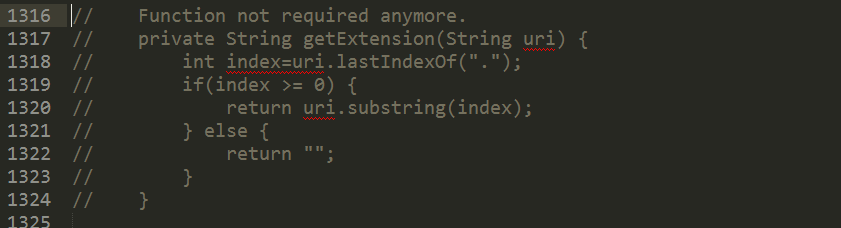
\includegraphics[width=\textwidth]{img/issue19.png}
    \caption{Commented out code}
    \label{fig:issue19}
\end{figure}

\issue[19]{Commented out sections} {
    There is only one function commented out: \code{getExtension} in line 1316 \
    (see figure~\ref{fig:issue19}).
    According to the comment above, the function is no more useful and can 
    be safely removed.  \\
    However, some snippets are commented out for reference and must not be 
    erased according to its comment (in lines 1146 and 1691). 
}

\begin{figure}[tb]
    \centering
    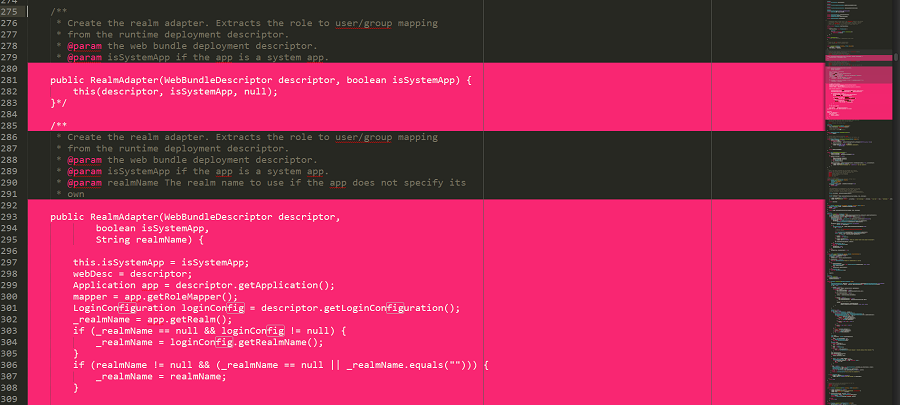
\includegraphics[width=\textwidth]{img/jdoc.png}
    \caption{Errors in Javadoc in lines 275--337}
    \label{fig:jdoc}
\end{figure}

\issue[23]{JavaDoc} {
    There are two wrong JavaDoc comments, shown in fig.~\ref{fig:jdoc}, 
    involving two constructors (lines 275--337). \\
    There are also a lot of methods without any JavaDoc comment.
    \begin{itemize}
    \item \code{WebBundleDescriptor}
    \item \code{getWebSecurityManager}
    \item \code{updateWebSecurityManager}
    \item \code{hasRole} (line 438)
    \item \code{doLogout} (line 489) 
    \item \code{authenticate} (line 518)
    \item \code{authenticate} (line 646)
    \item \code{authenticate} (line 661)
    \item \code{SecurityContext} (line 852)
    \item \code{SecurityContext} (line 856)
    \item \code{getPassword} (line 884) 
    \item \code{getPrincipal} (line 888)
    \item \code{getHostAndPort} (line 1147) 
    \item \code{redirect} (line 1250)
    \item \code{getCanonicalName} (line 1304) 
    \item \code{getResourceName} (line 1308)
    \item \code{setRealmName} (line 1343) 
    \item \code{validate} (line 1626)
    \item \code{shouldRegister} (line 1754) 
    \item \code{mapEntryToBoolean} (line 1762)
    \item \code{resetPolicyContext} (line 1790) 
    \item \code{getSecurityContextForPrincipal} (line 1959)
    \item \code{setCurrentSecurityContextWithWebPrincipal} (line 1977)
    \item \code{setCurrentSecurityContext} (line 1983)
    \item \code{initConfigHelper} (line 1988)
    \item \code{postConstruct} (line 1995)
    \end{itemize}
    
    Also, two inner classes: 
    \code{AuthenticatorProxy} (line 1798) and \\
    \code{HttpMessageInfo} (1846) have no JavaDoc comment.
}

\begin{figure}[htb]
    \centering
    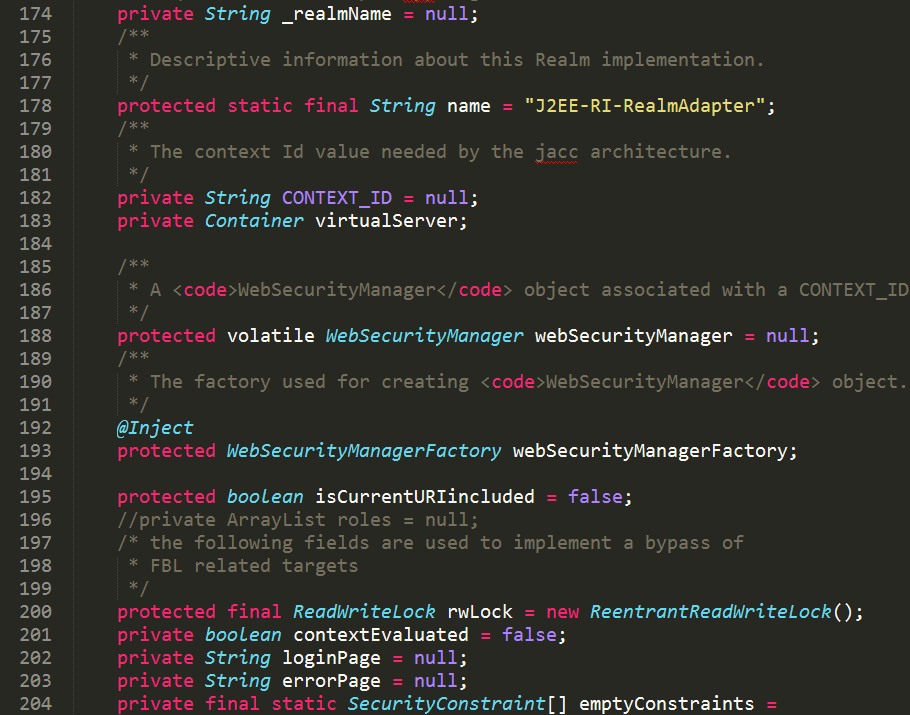
\includegraphics[width=\textwidth]{img/instancevariables.png}
    \caption{Protected and private variables are mixed}
    \label{fig:instancevariables}
\end{figure}

\issue[25]{Class declarations} {
    Points \textbf{A}, \textbf{B}, \textbf{C} are OK; \\ \\
    Point \textbf{D}: static variables are mainly grouped on top of 
    the class, few are mixed with non-static variables and methods, like \\
    \code{reentrancyStatus} in line 249, \code{CONF\_FILE\_NAME} and
    \code{HTTP\_SERVER\_LAYER} in line 1578. \\ \\ 
    Point \textbf{E}: instance variables are not 
    defined in the order shown in \cite{bib:assignment} 
    (see fig.~\ref{fig:instancevariables}), but are logically related. \\
    This means that some protected variables appear after private ones 
    (for example see lines 188--200). \\ \\ 
    Points \textbf{F} and \textbf{G}: As for the methods, constructors correctly appear before any 
    other method.
}

\issue[26]{Method organization} {
Methods seem to be logically grouped, even if some are out of order: 
\begin{itemize}
    \item Setting up WebSecurityManager (lines 368-400)
    \item Role checking (lines 400--444)
    \item Logout(lines 448--516) and Login (lines 518--714)
    \item Run-as functions(lines 715--963)
    \item Permission check functions (lines 965--1144)
    \item Host and port management (lines 1145--1247)
    \item Redirecting (lines 1250--1300)
    \item Getters \& setters (lines 1300--1350)
    \item Security constraints (lines 1356--1394)
    \item Pre and post auth methods (lines 1415--1575)
    \item Validation (lines 1626--1750)
    \item Other getter functions (lines 1754--1793)
    \item AuthProxy class (lines 1800--2000) 
\end{itemize}
}

\issue[27]{Long methods} {
    Here's a list of some quite long methods. 
    They should be split using helper methods.
    \begin{itemize} 
        \item \code{validate} (lines from 1626)
        \item \code{getHostAndPort} (lines from 1147)
        \item \code{invokeWebSecurityManager} (lines from 965)
        \item \code{authenticate} (lines from 518) 
    \end{itemize}
}

\subsection{authenticate()} % (fold)
\label{sub:auth}
\issue[13]{80 characters limit}{
    There are two lines that exceed the 80 character limit: the comment
    in line 687 and the line 688. 
}

\issue[18]{Comments} {
The JavaDoc comments explaining the method parameters are not up to date 
and seem to be misleading. No comments present in method, some may be useful 
to better explain the inner workings.
}

\issue[34]{Parameters order} {
    The parameters are not aligned with what explained in the JavaDoc above; 
    however, the list of parameters is sound and presented in a reasonable order (username, password, certificate). 
}

\issue[38]{IndexOutOfBoundExceptions} {
    There could be an overflow in line 684 but the exception is caught.
}

\issue[42]{Error messages} {
Error messages are not detailed and do not provide any guidance to 
how to solve problems (\code{web.login.failed} and \code{Exception} at
line 701 and 704).
}

\issue[52]{Exception handling} {
All code is wrapped in a try catch block; Exceptions are caught at a high level, 
which means they are all caught but handled in a very general way 
(see Point~42).
}

\subsection{preSetRunAsIdentity()}

\issue[5]{Method names should be verbs} {
    \code{Pre} is not a verb; the other words are with the first letter
    capitalized so that part is ok.
}

\issue[18]{Comments} {
JavaDoc is unclear, since it does not explain exactly when the function is 
called. The code in line 722 inside is self-explainatory, but something is 
not working regarding the principals (typed names) for a certain servlet, 
as the comments in line 752--755 state.
}
\issue[33]{Declarations at the beginning of blocks} {
Only one initialization in line 749, not on top of the block; however, 
this is due to the fact a check is performed before this instruction.
}

\subsection{postSetRunAsIdentity()}

\issue[5]{Method names should be verbs} {
    \code{Post} is not a verb; the other words are with the first letter
    capitalized so that part is ok.
}

\issue[13]{80 characters limit} {
    A comment in line 843 starts after the 80th character.
}

\issue[18]{Comments} {
    Comment in line 843 (\code{always null}) does not explain why it is so.
}

\issue[33]{Declarations at the beginning of blocks} {
    Variables defined just before use, not on top of block.
}

\issue[34]{Parameters order} {
    The parameters are not aligned with what explained in the JavaDoc above; 
    however, the list of parameters is sound and presented in a reasonable 
    order (username, password, certificate). 
}


\subsection{principalSetContainsOnlyAnonymousPrincipal()}
\issue[1]{Meaningful names} {
    Variable \code{rvalue} in line 868 has an unmeaningful name.
}

\issue[13]{80 characters limit}{
    Line 867 and line 869 exceed 80 character limit.
}

\issue[18]{Comments}{
    No comments, but code is self-explanatory.
}

\issue[36]{Return values}{
    As it might not seem, return value is coherently used during validation 
    in line 1684, where the principalSet is analyzed.
}
\subsection{invokeWebSecurityManager()}

\issue[13]{80 characters limit} {
    Lines 989 and 1031 exceeds 80 characters.
}

\issue[14]{120 characters limit} {
    Line 1031 exceeds 120 characters.
}

\issue[16]{Higher-level breaks} {
    In lines 965, 966, 967, 1003 and 1026 there are breaks which 
    are not ``higher-level'' breaks.
}

\issue[18]{Comments} {
    Few comments aside JavaDoc are present, but code is well-written 
    and comprehensible.
}

\issue[36]{Return values} {
The return value is used in two points where permission checking is needed: 
line 932 (\code{hasResourcePermission}, which wraps this function) 
and line 1432 (\code{preAuthenticateCheck}, to check if auth will actually 
be necessary). It is used correctly in both cases.
}

\issue[44]{Brutish programming} {
There are duplicate checks after line 1000. 
Lines from 1000 to 1020 could be improved by putting every
\code{\_logger.isLoggable(Level.FINE)} inside \\ \code{\_logger.fine()}.
}

\subsection{hasUserDataPermission()}
\issue[1]{Meaningful names} {
    Class variable \code{rvalue} in line 1140 has an unmeaningful name.
}

\issue[13]{80 characters limit}{
    Lines 1095, 1100, 1119, 1139 exceed 80 character limit.
}

\issue[14]{120 characters limit} {
    Line 1095 exceeds 120 characters.
}

\issue[16]{Higher-level breaks} {
In lines 1084, 1085, 1089, 1090 and 1139 there are breaks which are not
``higher-level''  breaks. \\
Also, the break in line 1139 is misplaced since a better positioning of it 
would have also solved the 80 chars exceeding problem.
}

\issue[33]{Declarations at the beginning of blocks} {
In general yes, except for initialization in line 1105, which is however done 
just before use in the subsequent block.
}

\issue[42]{Error messages} {
Error codes are delegated to HttpServletResponse, with a \code{BAD\_REQUEST}
or \code{FORBIDDEN} argument indicating that the request was not well-formed 
or not authorized (line 1119 and 1139 respectevely). \\ 
A warning is issued too with an error message and an ID in the first case.
}

\issue[52]{Exception handling} {
All IO exceptions are thrown out like the previous method. \\
An \code{IllegalArgumentException} indicating a bad request is caught 
and correctly handled.
}

% subsection authenticate (end)

\newpage
\section{Other issues}
% TODO AL E MATTIA: Vedi in cima a Google Docs per elenco bug
% -------> RICORDATEVI DI INSERIRE LE ORE ALLA FINE!!! :)

After a complete overhaul of the class in which our methods are placed, we have
spotted these bugs which can affect the proper behaviour of the class. \\ \\
According to the text comments in line 354, the method doesn't work properly 
because its run will result in a classload failure.
There is also a known bug (\texttt{no.4757733}) which affects the security 
context loading and saving. The issue can be shown in 
method~\texttt{preSetRunAsIdentity} starting in line 734 and in
method~\texttt{postSetRunAsIdentity} starting in line 827. \\ \\
The object passed in the two functions seems not to be the same, according to 
the JavaDoc comment in line 813, and this, in practical, forces the second 
method to always set the \texttt{SecurityContext} to NULL. \\ \\
Also, the comment in line 1124 says that there is a bug (\texttt{no.4947698}) 
in method~\texttt{hasUserDataPermission} (starting at line 1084), 
but an analysis of the given portion of the code does not seem 
to enlighten any issue.

\appendix

\clearpage
\addcontentsline{toc}{section}{References}

\begin{thebibliography}{9}
\bibitem{bib:assignment} Prof. Di Nitto.
\emph{Assignment 3: Code Inspection}.

\bibitem{bib:docurl} AA.VV.,
\emph{Java EE 6 Official Documentation}.
\url{https://docs.oracle.com/javaee/6/tutorial/doc/bnbxj.html}

\bibitem{bib:javadoc} AA.VV.,
\emph{GlassFish Appserver Parent Project 4.1.1 API - Javadoc}.
\url{http://glassfish.pompel.me/}
\end{thebibliography}

\end{document}
